\documentclass[11pt]{article}
\usepackage{graphicx}
\usepackage{hyperref}
\usepackage{amsmath}
\usepackage{amsthm}
\usepackage{amssymb}
%\usepackage[all=normal,floats,leading,paragraphs,charwidths,tracking,wordspacing]{savetrees}
\usepackage{float}
%\usepackage[version = 4]{mhchem}
\usepackage{multirow}
\usepackage{commath}
\usepackage{booktabs}
\usepackage{subcaption}
\usepackage{natbib}
\renewcommand{\arraystretch}{1.2}
\usepackage{setspace}
\onehalfspacing
\usepackage[nottoc,numbib]{tocbibind}
\usepackage{siunitx}
\sisetup{detect-all}
\DeclareSIUnit{\atm}{atm}
\usepackage{listings}
\usepackage{color} %red, green, blue, yellow, cyan, magenta, black, white
\definecolor{mygreen}{RGB}{28,172,0} % color values Red, Green, Blue
\definecolor{mylilas}{RGB}{170,55,241}
\usepackage[a4paper,margin=20mm]{geometry}
\numberwithin{equation}{section}
\setlength{\parskip}{\baselineskip}
\setlength{\parindent}{0pt}
\hypersetup{
    colorlinks=true,
    linkcolor=black,
    filecolor=black,      
    urlcolor=black,
    citecolor=black
}
\urlstyle{same}
\lstset{language=Matlab,%
    %basicstyle=\color{red},
    breaklines=true,%
    morekeywords={matlab2tikz},
    keywordstyle=\color{blue},%
    morekeywords=[2]{1}, keywordstyle=[2]{\color{black}},
    identifierstyle=\color{black},%
    stringstyle=\color{mylilas},
    commentstyle=\color{mygreen},%
    showstringspaces=false,%without this there will be a symbol in the places where there is a space
    numbers=left,%
    numberstyle={\tiny \color{black}},% size of the numbers
    numbersep=9pt, % this defines how far the numbers are from the text
    emph=[1]{for,end,break},emphstyle=[1]\color{red}, %some words to emphasise
    %emph=[2]{word1,word2}, emphstyle=[2]{style},    
}
\begin{document}
\begin{titlepage}
    \begin{center}
        \vspace*{1cm}
             
        MECH0020 Individual Project\\
        2021/22
 
        \vspace{1.5cm}

        {\LARGE \textbf{Designing a Lap Simulator for the Shell Eco-marathon} \par}
             
        \vspace{1.5cm}
 
        Student: Hasha Humayon Dar
        
        \vspace{0.25cm}

        Supervisor: Professor Tim Baker

        \vspace{0.25cm}

        Word count: FILL
        
        \vfill

        University College London\\
        Torrington Place\\
        LONDON WC1E 7JE
             
    \end{center}
 \end{titlepage}
\newpage
\section*{Declaration}
I, Hasha Humayon Dar, confirm that the work presented in this report is my own. Where information has been derived from other sources, I confirm that this has been indicated in the report.
\section*{Abstract}
The development of simulating performance parameters for racing vehicles has become increasingly important in a digital world. Simulations provide highly customisable virtual environments to test components, changes and strategies. Hence, the development of software that can give an accurate idea of a vehicle's performance in a variety of configurations would prove to be an advantage. Traditionally, the UCL Racing Team has conducted in-person testing of their vehicles at race tracks or similar. However, due to COVID-19, this has become difficult in the past two years. Virtual testing can provide a cheaper, more time efficient means of testing. The development of a virtual model of the vehicle would allow the team to test various changes to the vehicle, without having to prototype and arrange for in-person testing. 

This report focuses on building a performance based model of the UCL Racing Shell Eco-marathon vehicle, which generates a lap time for the vehicle. The Shell Eco-marathon is a competition at the school and university level for students focusing on energy optimisation in vehicles. The aim of the competition is to develop new innovations in energy efficiency for vehicles on the road with the idea of reducing carbon emissions \citep{shell1}.
\section*{Acknowledgements}
Throughout this project I have received a great deal of support and assistance. First and foremost, I would like to thank my supervisor, Prof. Tim Baker, whose expertise was invaluable in the development of this project. 

I would also like to acknowledge the support of the UCL Mechanical Engineering Department, which champions innovation through projects like these. Their facilities and teaching have proven to be an incredible asset for this project. 

I would also like to thank my parents for their continuous and unwavering support of my studies and activities. Thank you for always being there for me. Finally, there are my friends, who were a source of support and distraction, both of which proved very useful for deliberating over problems and to rest my mind from academia. Thank you to you all.
\newpage
\tableofcontents
\listoffigures
\listoftables
\newpage
\section{Introduction}
\subsection{Project background and problem}
UCL Racing currently competes in the Shell Eco-marathon in the `prototype' category. Hence, this simulator will focus on reproducing the performance characteristics of a vehicle in this class. The vehicles is a small hydrogen-powered single-seater, designed with a focus on attaining ultra-efficiency through the optimisation of the aerodynamic and performance characteristics of the vehicle.

For an ultra-energy-efficient vehicle, there are many sources of inefficiency. Some of them are aerodynamic drag (air resistance), friction drag (from the road surface) and losses in the powertrain (electricity generation, mechanical losses) \citep{Wei2019}. The design itself of the car must be optimised to increase its performance such as the weight of the vehicle \citep{Tsirogiannis2019}.

A problem that arises when investigating and modelling these variables is that there is no way of testing certain performance characteristics within the holistic context of the competition virtually. Currently, to test newly designed components and its overall impact on the performance of the vehicle, the part must be prototyped and installed on the vehicle, and then experimentally tested. This presents a problem as this is costly, time-consuming and constrains the number of prototypes that can be made.

A transient, dynamic lap simulator will allow the analysis of the vehicle's various performance characteristics. This will allow the team to optimise and prototype designs much more effectively. The team would be able to test the vehicle on the final test track, without the cost of being there physically. This simulator will also allow vehicular strategies to be tested, as virtually any track can be inputted and tested. 

As creating a virtual model of a vehicle can become an extremely complex process depending on the resolution and level of accuracy required. This simulator will focus specifically on the overall performance parameters of the vehicle, considering the car as a homogeneous unit, rather than an assembly of the various components that make up a vehicle. 
\subsection{Objectives}
The simulator should meet the following objectives:
\begin{itemize}
    \item Process and store track data
    \item Process and store vehicle data
    \item Calculate forces acting upon the vehicle and sources of inefficiency during a transient simulation of the vehicle running around the track.
    \item Output data on various performance parameters
    \item Generate a lap time for the vehicle
\end{itemize}
As this simulator is designed to be used by students in the coming years as tool to inform them on their design choices, an element of ease of use is also important. Good practices such as well written and laid out code is important to ensure that outside users can understand it and make their own adjustments. The software should also be computationally efficient, allowing for use on most machines without requiring large amounts of computer resources. 
\section{Literature review}
\section{Methodology and design}
\subsection{Track data}
It was decided that a simulator which can simulate a vehicle for any track was important to allow for a wider array of testing scenarios. Hence, the simulator is designed to use only x-y-z-coordinate data as an input. Calculations are then made on various aspects of the track. This includes the radius of curvature of the track, which is calculated using geometrical principles.
\begin{figure}[H]
    \centering
    
\includegraphics[width = 0.8\textwidth]{./img/radiusOfCurvature.png}
    \caption{Radius of curvature calculation.}
\end{figure}
The code indexes the x-y coordinates of three sequential track points and calculates the radius of curvature by use of the following equations.
\begin{gather}
    a = \sqrt{\left(x_2 - x_1\right)^2 + \left(y_2 - y_1\right)^2}\\
    b = \sqrt{\left(x_3 - x_2\right)^2 + \left(y_3 - y_2\right)^2}\\
    c = \sqrt{\left(x_3 - x_1\right)^2 + \left(y_3 - y_1\right)^2}\\
    q = \dfrac{a^2 + b^2 - c^2}{2ab}\\
    R = \dfrac{c}{2\sqrt{1 - q^2}}
\end{gather}
\begin{figure}[H]
    \centering
    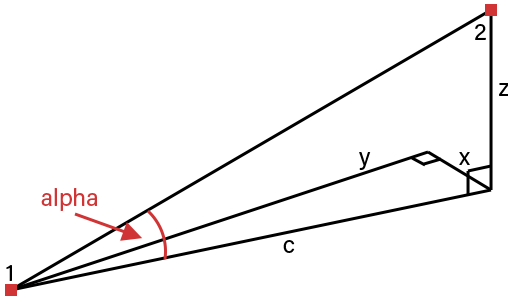
\includegraphics[width = 0.6\textwidth]{./img/trackSlope.png}
    \caption{Track slope calculation.}
\end{figure}
The slope between adjacent track points is calculated using trigonometry.
\begin{gather}
    c = \sqrt{\left(x_2 - x_1\right)^2 + \left(y_2 - y_1\right)^2}\\
    z = z_2 - z_1\\
    \alpha = \arctan\left(\dfrac{z}{c}\right)
\end{gather}
After the calculation of the radius of curvature and slope at the discrete steps along the length of the track, these values are concatenated with the cumulative distance of the track. This will allow us to interpolate the values of the above variables during our simulation. 
\subsection{DC motor model}
The car is powered by a small DC motor, attached to the rear wheel. A Simscape DC motor model was used to output torque as function of a virtual throttle position. This allows for a highly customisable power unit and control system.
\begin{figure}[H]
    \centering
    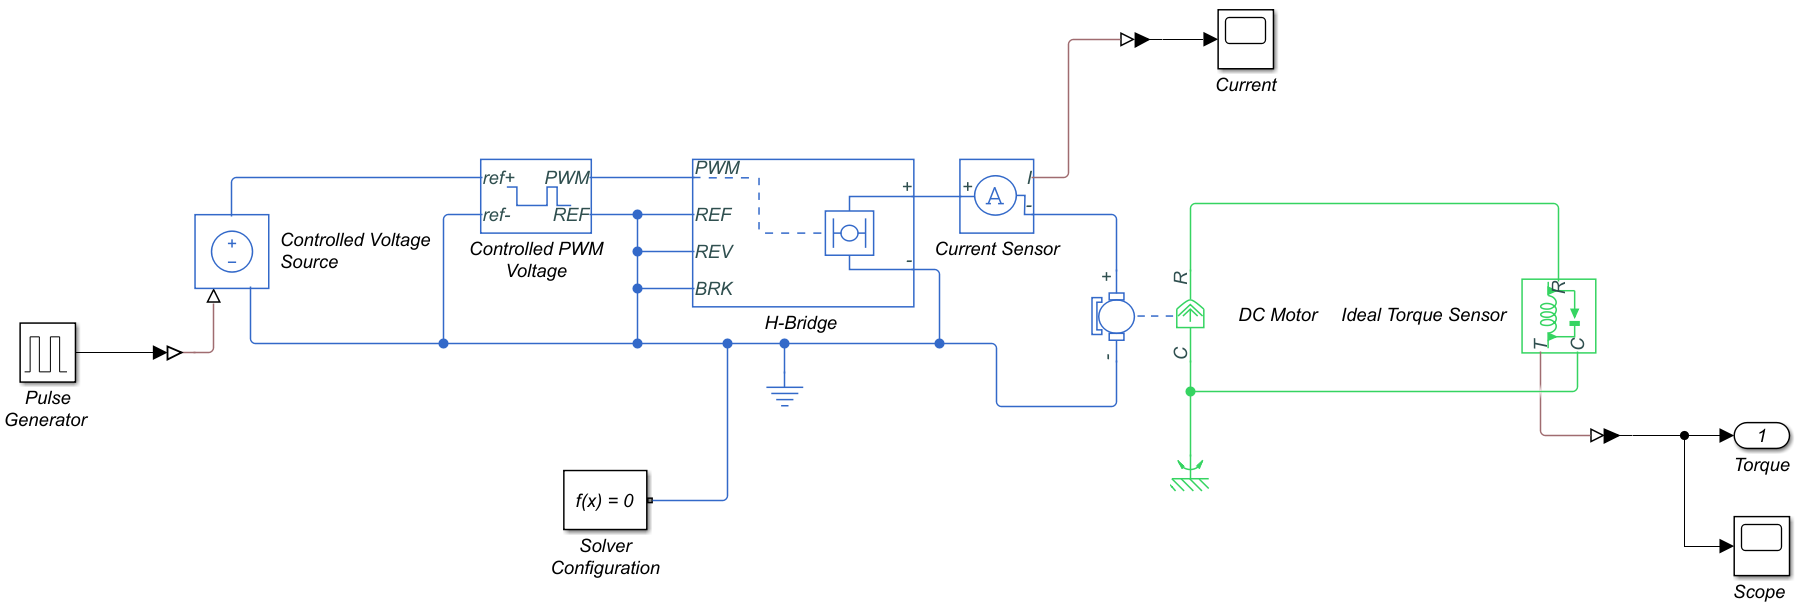
\includegraphics[width =\textwidth]{./img/DCMotorModel.png}
    \caption{DC motor model.}
\end{figure}
The throttle input can be inputted into the simulation via the use of an array as a function of the time. A PWM controller is then used as an input to the motor driver, which provides current to the DC motor. The Simscape DC motor block allows the motor parameters to be defined as a function of the rated load and speed. Electrical characteristics such as the armature inductance, and rated supply voltage are defined here as well. Mechanical characteristics such as the rotor inertia and damping can also be added. A torque sensor is then used to provide our output.
\subsection{Transmission model}
The Shell eco car utilises a simple transmission with only one drive ratio. Transmission inefficiencies stemming from mechanical losses can be modelled using a variable gain factor. The drive ratio converts the torque from the DC motor shaft to the torque applied at the wheel.
\begin{figure}[H]
    \centering
    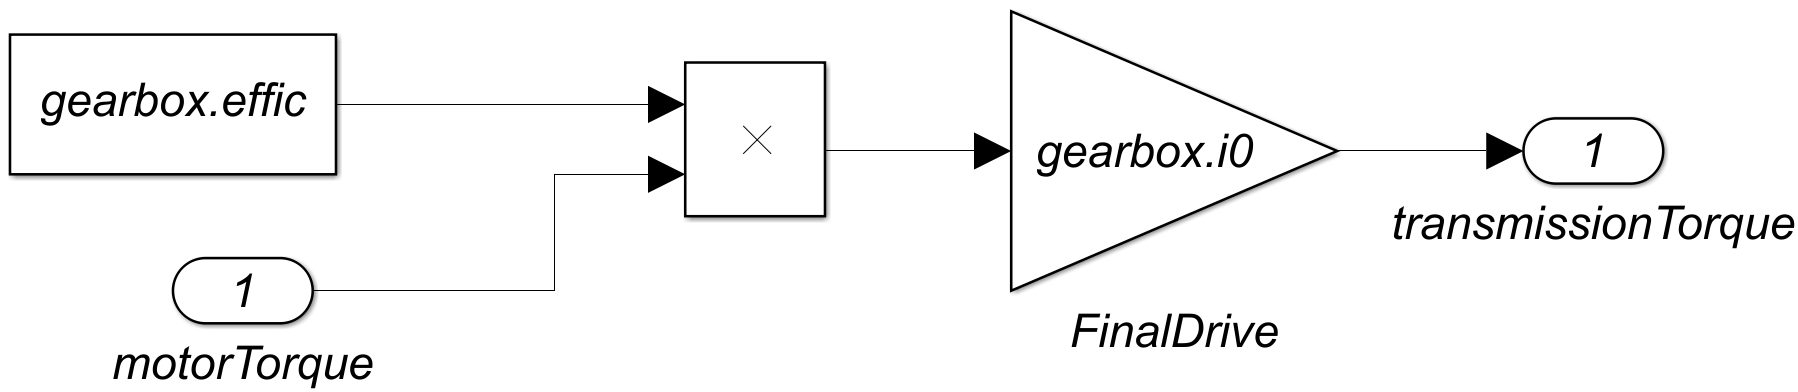
\includegraphics[width =\textwidth]{./img/transmissionModel.png}
    \caption{Transmission model.}
\end{figure}
\subsection{Vehicle model}

\section{Model validation and results}
\section{Discussion}

\newpage
\bibliographystyle{agsm}
\bibliography{./bib/MECH0020refs.bib}
\end{document}